\documentclass{standalone}
\usepackage{tikz}
\usepackage{ctex,siunitx}
\setCJKmainfont{Noto Serif CJK SC}
\usepackage{tkz-euclide}
\usepackage{amsmath}
\usepackage{wasysym}
\usetikzlibrary{patterns, calc}
\usetikzlibrary {decorations.pathmorphing, decorations.pathreplacing, decorations.shapes,}
\begin{document}
\small
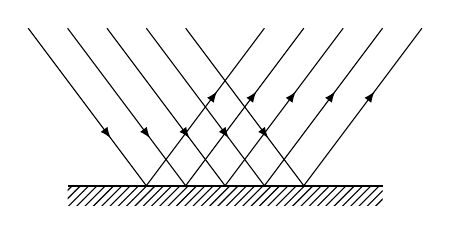
\begin{tikzpicture}[>=latex]
  \foreach \x in {-1,-0.5,0,0.5,1}
  {
      \draw[postaction={decorate},decoration={markings,mark={between positions 0.35 and 0.9 step 0.45 with {\arrow{>}}}}] (\x-1.5,2.0)--(\x,0)--++(1.5,2.0);
  }
  \fill [pattern=north east lines] (-2,-.25) rectangle (2,0);
  \draw [thick](-2.0,0)--(2.0,0);
\end{tikzpicture}
\end{document}